%%%%%%%%%%%%%%%%%%%%%%%%%%%%%%%%%%%%%%%%%%%%%%%%%%%%%%%%%%%%%

\mainmatter
\setcounter{page}{1}

\lectureseries[\course]{\course}

\auth[\lecAuth]{Lecturer: \lecAuth\\ Scribe: \scribe}
\date{November 10, 2009}

\setaddress

% the following hack starts the lecture numbering at 13
\setcounter{lecture}{12}
\setcounter{chapter}{12}

\lecture{Convergence \& Consistency}

\section{Prediction Review}
In Lecture 11 (\ref{eq:error}) showed that the prediction error is
\begin{align*}
\epsilon(t,\theta) &= H_0^{-1}(q)[y(t)-G_0(q)u(t)] \\
\hat{\theta} &= \arg\min_\theta\frac{1}{N}\sumt\epsilon^2(t,\theta)
\end{align*}

In Table \ref{tab:models} we looked at different model strutures to parameterize $G_\theta$ and $H_\theta$, some of which were ARX, ARMAX, OE, BJ, PEM. We saw that conventional least squares is equivalent to using PEM+ARX.  The structural parameters for these models were given as $n_a$, $n_b$, $n_c$, $n_d$, $n_f$ and $n_k$.

\section{Convergence \& Consistency for PEM Model}
This section corresponds to Chapter 8 in Ljung. See Figure \ref{fig:13overview} to see how models are typically used and validated. If the model is not validated then we can go back and modify our experiments to collect new or more data. The model $M(\theta)$ needs prior assumptions about what noise model structure will be used and the order of the noise/system. Optimization can be performed using conventional, time-weighted or constrained least squares approaches or even quadratic programming. When attempting to validate a model we typically assume that $u(t)\perp e(t)$. The validation process usually involves checking to see if $e(t)$ or $\epsilon(t,\theta)$ are white noise. If they are white it means that we have extracted all of the useful information out of the system and the model is a good fit, see \S\ref{sec:generalpredictor} for more details.

\begin{figure}[ht!]
	\centering
	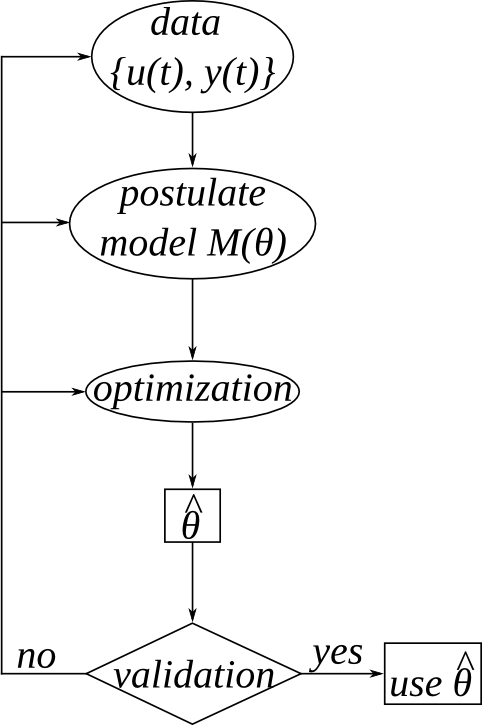
\includegraphics[width=.5\textwidth]{images/13overview}
	\caption{Overview of identifying parameter estimates.}
	\label{fig:13overview}
\end{figure}

A model is consistent if $\mathcal{S}\in\mathcal{M}$. A model converges if $\lim_{N\to\infty}\hat{\theta}^N = \theta_0$ w.p. $1$. We will use the steps in Figure \ref{fig:13overview} to look at these properties of models. First we have to make some assumptions.

\subsection{Assumptions on Data}

%%%%%%%%%%%%%%%%%%%%%%%%%%%%%%%%%%%%%%%%%%%%%%%%%%%%%%%%%%%%%